
\documentclass[preprint,12pt]{elsarticle}

\usepackage[spanish]{babel}
\usepackage{amssymb}
\usepackage{graphicx}
\usepackage{lineno}
\usepackage[utf8]{inputenc}
\usepackage{url}
\usepackage{natbib}

\begin{document}
	
	\begin{frontmatter}

		\title{\huge  RETOS Y OPORTUNIDADES DE DEVOPS EN LA BASE DE DATOS}
		
		\author{Robles Flores, Anthony Richard	              (2016056192)}
		\author{Porlles Carrillo, Diego Armando              (2015050948)}
		\author{Sandoval Blas, Jesus Enrique           (2016054467)}
		\author{Quispe Mamani, José Luis              (2015053235)}
		
		\address{Tacna, Perú}
		
		\begin{abstract}
			%% Text of abstract
DevOps is a conceptual framework for reintegrating development and operations of Information Systems. We performed a Systematic Mapping Study to explore DevOps. 26 articles out of 139 were selected, studied and summarized. Based on this a concept table was constructed. We discov-ered that DevOps has not been adequately studied in scientific literature. There is relatively little research available on DevOps and the studies are often of low quality. 
\\
\\
We also found that DevOps is supported by a culture of collaboration, automation, measurement, information sharing and web service usage. DevOps benefits IS development and operations performance. It also has positive effects on web service development and quality assurance performance. Finally, our mapping study suggests that more research is needed to quantify these effects.
		\end{abstract}
\end{frontmatter}
%%
	%% Start line numbering here if you want
	%%
	%\linenumbers
	
	%% main text
	\section{Resumen}

DevOps es un marco conceptual para reintegrar el desarrollo y las operaciones de los sistemas de información. Realizamos un estudio de mapeo sistemático para explorar DevOps. 26 artículos de 139 fueron seleccionados, estudiados y resumidos. En base a esto, se construyó una tabla conceptual. Descubrimos que DevOps no se ha estudiado adecuadamente en la literatura científica. Hay relativamente poca investigación disponible sobre DevOps y los estudios a menudo son de baja calidad. 
\\
\\
También descubrimos que DevOps está respaldado por una cultura de colaboración, automatización, medición, intercambio de información y uso de servicios web. DevOps beneficia el desarrollo de IS y el rendimiento de las operaciones. También tiene efectos positivos en el desarrollo del servicio web y el rendimiento del aseguramiento de la calidad. Finalmente, nuestro estudio de mapeo sugiere que se necesita más investigación para cuantificar estos efectos.
%%https://www.researchgate.net/publication/267330992_Report_DevOps_Literature_Review



%%INTRODUCCION%%-------------------------------------------------------------------------------------------
\section{Introducción}
El desarrollo ágil divide en iteraciones el desarrollo de un sistema software para
obtener incrementos de software funcional. A pesar de los beneficios del desarrollo
ágil, se originan nuevos retos debido a las brechas que aparecen al momento de integrar, realizar pruebas y desplegar a producción cada incremento. Además, el tiempo
de entrega de cada incremento es un factor importante que origina una ventaja compe-
titiva a las organizaciones, permitiendo obtener retroalimentación de los clientes y de
esta manera realizar una mejora continua de los productos de software.
Realizar manualmente los procesos de integración, pruebas y despliegue de incrementos de software ocasiona en la mayoría de los casos retrasos en la planificación de
los proyectos y es propenso a errores con un resultado no confiable
\\
\\
DevOps es un
conjunto de principios y prácticas que optimizan el tiempo de entrega de software,
gestionan la infraestructura como código y mejoran la experiencia del usuario en base
a la retroalimentación de sus comentarios. Las prácticas de DevOps  son:
 i) la integración continua construye todo el software y ejecuta un conjunto de pruebas con
cada incremento, ii) el despliegue continuo toma el software creado en la integración
y lo despliega en un entorno de operaciones de una manera automática, y iii) la entrega continua proporciona la capacidad de liberar en el entorno de operaciones nuevas
versiones de software varias veces al día.
\\
\\
Es un método de reconfiguración dinámica incremental de arquitecturas
de servicios cloud basado en el Desarrollo de Software Dirigido por Modelos
(DSDM). Este método tiene como objetivo apoyar a los desarrolladores de software
en la integración incremental de servicios en entornos cloud, por tal motivo provee un
conjunto de actividades que soportan: i) el diseño de la integración, ii) la implementación de la integración, y iii) el despliegue y reconfiguración arquitectónica.
%%-------------------------------------------------------------------------------------------

%MARCO TEORICO-------------------------------------------------------------------------------------------
\section{Marco Teórico}

\subsection{Definición}

DevOps es una metodología de desarrollo de software que apunta a reunir equipos de desarrollo de software y operativos de tecnología de la información. Es un concepto que fomenta una cultura de colaboración entre estos dos equipos que históricamente trabajaron en sus propios silos separados, desde la fase de diseño inicial hasta el lanzamiento del producto.

DevOps es una metodología que combina el desarrollo de software (Dev) con las operaciones (Ops). La intención es permitir la comunicación entre los equipos para que puedan construir, probar y lanzar software más rápidamente y con mayor eficiencia y velocidad.

Al combinar estos dos equipos y procesos distintos, se promueve la integración continua, la implementación continua, las pruebas automatizadas y la transparencia en los repositorios de código.


\cite{DWarehouse02}
\\
\\

\begin{figure}[htb]
				\begin{center}
					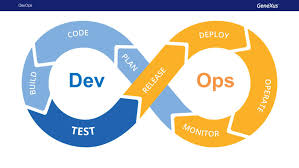
\includegraphics[width=9cm]{./IMAGENES/definicionsql}
				\end{center}
			\end{figure}

\subsection{¿Qué es Agile?}
La metodología ágil es también una metodología de desarrollo de software que surgió alrededor del año 2001, cuando se presentó el manifiesto ágil. Emplea cuatro valores y doce principios que ayudan a construir una cultura de desarrollo de software "ágil".

En términos generales, ágil fomenta la adopción y una mentalidad de liderazgo que promueve el trabajo en equipo, la autoorganización y la responsabilidad. Más importante aún, el enfoque ágil se enfoca más en alinear continuamente el desarrollo con las necesidades y tendencias del cliente, incluso cuando esas necesidades y tendencias cambian al final del proceso de desarrollo.
\\
\\
Agile incorpora un conjunto de principios que ayudan a individuos, equipos y unidades más grandes a trabajar juntos. La "mentalidad ágil" se enfoca más en las personas que en los procesos y herramientas. Una organización ágil se adapta y aprende sobre el cambio constante que les permite identificar nuevas oportunidades y añadir más valor para los clientes. "SQL-92" o "SQL2".\cite{DWarehouse02}
\\
\\

\begin{figure}[htb]
				\begin{center}
					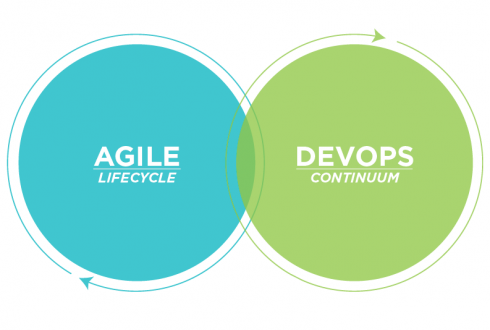
\includegraphics[width=10.5cm]{./IMAGENES/evolucion}
				\end{center}
			\end{figure}


\subsection{Requisitos para implementar una cultura DevOps}
Lo primero es comunicar que la cultura DevOps se va a implementar, mencionando los beneficios y haciendo que el equipo se sienta parte del cambio. Luego explicar las acciones que se van a tomar, no importa que no sean desarrolladores.

La comunicación y colaboración para tener una cultura DevOps son cruciales, es un trabajo entre los desarrolladores y los equipos encargados de la infraestructura de los servidores.

La tarea principal será la automatización, reducir los tiempos de despliegue del producto y mantener una calidad de desarrollo y estabilidad para el usuario. Debes tener claro que esto será un proceso sin fin, por lo que cada mejora te dará el tiempo que dedicarás para innovar el proceso y hacerlo cada vez mejor.
%%-------------------------------------------------------------------------------------------


%CONCLUSIONES-------------------------------------------------------------------------------------------
\section{Conclusiones}

\subsection{Conclusión 1 : }	
Con sql nos permite ingresar comandos o sentencias de tal manera que podemos administrar o crear una base de datos.
Es la variedad de comandos que nos permiten generar datos desde la creación, modificasion o mantenimiento a las tablas las cuales también nos permiten recuperar datos o importarlos de siferentes maneras.

\subsection{Conclusión 2 : }	
Es difícil imaginar hoy en dia la concentración de información sin base de datos, las pequeñas o grandes industrias tienen como base su sistema informatico la construcción de base de datos con las que podemos tener una gran versatilidad incluso con los equipos myframe.
La seguridad en las bases de datos es muy importante debido a que garantiza la integridad física y la lógica de los datos de información.

%%-------------------------------------------------------------------------------------------

%%
	
	%%
	%\linenumbers
	
	%% main text

	
	\newpage
	
	\bibliographystyle{apalike} 	%ESTILO
	\bibliography{BIBLIOGRAFIA}	 
\citep{DLake01}  
\citep{DLake02}  
\citep{DWarehouse01}  
\citep{DWarehouse02}   
	

\end{document}

